\documentclass{article} % For LaTeX2e
\usepackage{neurips,times}
\usepackage{hyperref}
\usepackage{url}
\usepackage{booktabs}       % professional-quality tables
\usepackage{graphicx}
\usepackage{lipsum}
\usepackage{amsmath}
\usepackage{multirow}
\usepackage{pgfplots}
\pgfplotsset{compat=newest}

\usepackage[utf8]{inputenc} % allow utf-8 input
\usepackage[T1]{fontenc}    % use 8-bit T1 fonts
\usepackage{hyperref}       % hyperlinks
\usepackage{url}            % simple URL typesetting
\usepackage{booktabs}       % professional-quality tables
\usepackage{amsfonts}       % blackboard math symbols
\usepackage{nicefrac}       % compact symbols for 1/2, etc.
\usepackage{microtype}      % microtypography
\usepackage{amssymb,amsmath,bm}
\usepackage{color,soul}
\usepackage{multirow}
\usepackage{mathtools}
\usepgfplotslibrary{groupplots}


\def\figwidth{.5\linewidth}
\def\figheight{.15\textheight}
%\newlength{\figwidth}{\mywidth}
%\newlength{\figheight}{.2\textheight}


\usepackage[numbers]{natbib}
\setlength{\bibsep}{0.0pt}

\title{Unsupervised Learning of Disentangled and Interpretable Representations from Sequential Data\\ \vspace{0.5cm}\large{Report}}
\author{Stefan Wezel \\ stefan.wezel@student.uni-tuebingen.de \\4080589  \\ ML4S}

\newcommand{\fix}{\marginpar{FIX}}
\newcommand{\new}{\marginpar{NEW}}

\nipsfinalcopy

\begin{document}
%\setlength{\figwidth}{.8\textwidth}
%\setlength{\figheight}{.2\textheight}
\maketitle

\begin{abstract}
%Sequential data often has the intrinsic quality of containing information playing out on multiple time scales. Features can appear low frequencies and on high frequencies. 

%
%While Variational Autoencoders (VAE) have proven to be a successful methodology on i.e. image data, 



Information in sequential data is often distributed over multiple time scales.
While if viewed as a single signal, such data might appear noisy. However, patterns can emerge if temporal scales are inspected separately from one another.
\citet{hsu2017unsupervised} leverage this intrinsic structure to learn disentangled representations from sequential data in an unsupervised manner with a proposed factorized hierarchical variational autoencoder (FHVAE). They aim to factorize sequence level and segment level attributes into distinct latent subspaces. Architectural and sequence-dependent priors create an inductive bias to encourage the proposed factorization. Here, we put their work into a formal context, explore the proposed methodology, and reflect critically on their work \footnote{An implementation of \citet{hsu2017unsupervised}'s method and our experiments can be found at \url{www.github.com/wastedsummer/SequentialVAE}}.
\end{abstract}

\section*{Introduction}
Intuitively, disentangled representations are representations that are reflective of the underlying generating factors of observed data in thus they are encoded as separate latent subspaces (See Figure~\ref{fig:intuition}). This notion is already present in classical factor analysis work, where it is referred to as independent component analysis (ICA) \cite{comon1992independent}.\\
However, many problems cannot be solved in a linear fashion. The success of deep neural networks (DNN) can be largely attributed to the fact that they are very powerful non-linear function approximators. Thus, making them a promising method to solve the long-standing problem of non-linear ICA.\\
Different methods have been proposed to learn such disentangled representations \cite{higgins2016beta, chen2016infogan, kulkarni2015deep} with varying success. Many of these works focus on image data. However, it has been shown by \citet{locatello2019challenging} that disentangled representations cannot be learned without introducing any kind of supervision or inductive biases. Sequential data, while having been explored less, offers an inherent structure that can be exploited to construct inductive biases as has been proposed by \citet{hsu2017unsupervised}.\\
Besides technical challenges, this strain of research suffers from the lack of formally defined and agreed upon foundations. The very term of disentangled representations for example is often understood differently in between works. In the following section, we will use the definition proposed by \citet{higgins2018towards} to put the work by \citet{hsu2017unsupervised} into formal context.

\begin{figure}
	\centering
	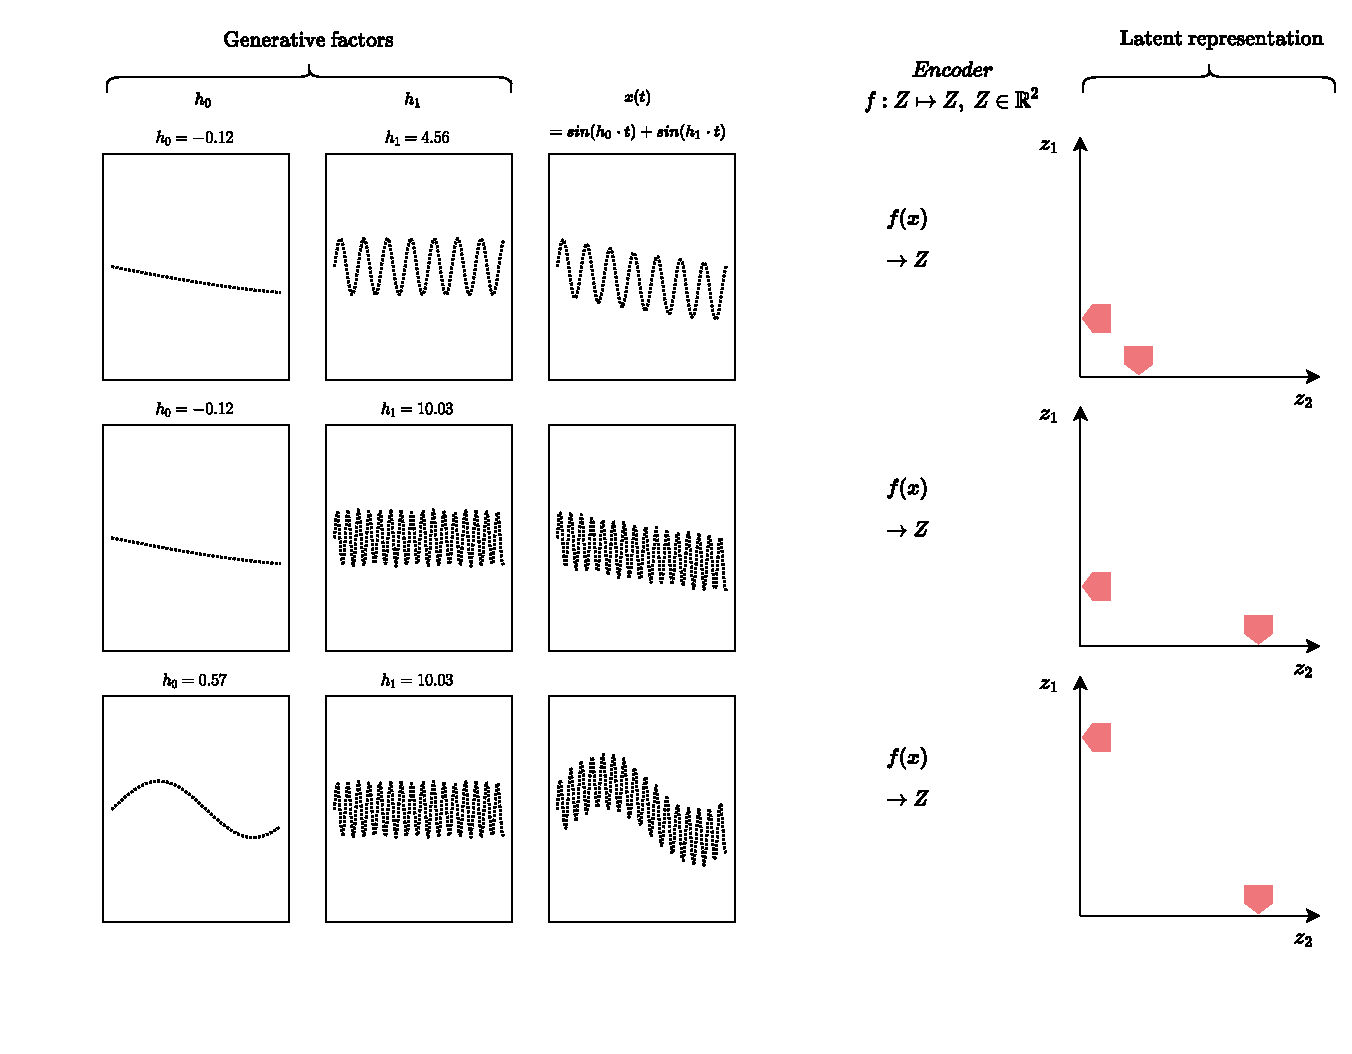
\includegraphics[width=.9\linewidth]{../figures/intution_3x3_static.pdf}
	\caption{Changing values of generating factors are reflected in the corresponding latent variables.}
	\label{fig:intuition}
\end{figure}


\section*{Viewing the FHVAE though a Formal Lense}
Works on disentanglement often lack a proper formal framework \cite{higgins2018towards}. While claiming to achieve disentanglement, \citet{hsu2017unsupervised} do not provide any formal foundation for their claim. With no formal tools at hand, we cannot formally discuss whether disentanglement was achieved. Thus, we use the following sections to give a theoretical background that defines disentanglement in group-theoretic terms, and describe the problem, the FHVAE was designed to solve, using the established formal framework.



\subsection*{The Tools of Group Theory}
A group is described by a tuple of an operation $\circ$ and a non-empty set $G$. The set has to be closed under the operation, it must contain an identity element, the operation must be associative, and for every element in $G$, there must be an inverse element \cite{benkart1987abstract}.
Multiple groups $G_i$ can be combined via a direct product $G = G_1 \times ... \times G_n$. The result of this direct product is itself a group.\\%, where operations $\circ_{G_i}$ act each respective sets $G_{G_i}$ of each subgroup.
Groups that are of particular interest for the field of disentangled representation learning are symmetry groups \cite{benkart1987abstract}.
A symmetry group consists of a set of transformations that leave a given object $X$ invariant. Its operation is the composition of such transformations. A prominent example of a symmetry group is $SE_3$. This symmetry group can be visualized as a set set of vertices $X$ that form an equilateral triangle. Permutations of this set would result in rotations or flips of the triangle. These permutations would be the symmetry transformations of our symmetry group. The operation would be composing multiple permutations.\\
Another important concept is the group action. It is the result of applying a symmetry transformation to an object. In our triangle example, a group action would be the permuted set of vertices.\\
If a group action on $X$ is the result of a subset $G_i$ of symmetries $G= G_1 \times ... \times G_n$ and only affects a subset $X_i$ of $X$ but leaves all other $X_{j\neq i}$ unchanged, we say it is a disentangled group action. Such disentangled group actions are of particular interest for disentangled representation learning, and generally are what we want to model. Note, that if we observe such disentangled group actions, we can infer that $G$ can be decomposed into a direct product of symmetry groups $G_i$ without knowing the underlying processes.\\
To model such a process, we need to find some symmetry preserving mapping $f:X\mapsto Z$. It should not matter, whether $X$ is mapped to $Z$ followed by applying a symmetry $G$ or $G$ is applied to $X$ and then mapped to $Z$. The resulting space $Z$ should be the same. This is visualized below.
\begin{align*}
%\begin{align}
&X \;\xrightarrow[\text{}]{G}\;\;X\\ 
f&\downarrow \;\;\;\;\;\;\;f\downarrow\\
&Z \;\xrightarrow[\text{}]{G}\;\;\;Z
\end{align*}
Such a mapping is called an equivariant map. Its result is a disentangled representation. The space $Z$ (which we will also refer to as latent space in the following) naturally decomposes into a direct product of independent subspaces $Z_1 \times ... \times Z_n$. Moreover, each subspace $Z_i$ is only affected by symmetry $G_i$ on $X$ (as only $X_i$ is changed) and remains invariant to all other $G_{j \neq i}$.\\
Note that it is only disentangled with respect to a certain decomposition. This is important, as it means we can only discuss whether disentanglement was achieved if the decomposition is sufficiently clear. Not all decompositions make sense or are possible to model.\\
As these concepts are rather abstract, we will use the next section to frame the real-world setting of \citet{hsu2017unsupervised} using group-theoretic terms to build further intuition and a formal foundation to discuss their work.


\subsection*{Symmetries in Sequential Data}
\citet{hsu2017unsupervised} argue that certain sequential data can be factorized into attributes of different temporal scales. For example, voice recordings can be decomposed into sequence attributes and segment attributes. In this context, sequence attributes are features that remain unchanged over multiple sequences if spoken by the same speaker. Segment attributes, on the other hand, vary in sequences and are independent of the speaker. They are determined by variables such as linguistic content.\\
In group-theoretic terms, we could state this as the group $G$ acting on audio recordings $X$ is a direct product of $G_{sequence} \times G_{segment}$, because we observe the resulting disentangled group actions of this decomposition. \citet{hsu2017unsupervised} now want to find a representation that is disentangled with respect to this decomposition. They need to find an equivariant map $f:X\mapsto Z$, where $Z = (z_1, z_2)$ is a latent space, so that i.e. $z_2$ is only affected by $G_{sequence}$ and $z_1$ only is affected by $G_{segment}$. Then, the proposed decomposition of symmetries is reflected in $Z$.\\
For this specific setting, finding such an equivariant map would allow separating speaker information from content information. This in turn would enable us to reconstruct given content information using another speaker's voice information. \citet{hsu2017unsupervised} propose this as a qualitative assessment of their disentanglement. Quantitative evaluation of disentanglement is notoriously challenging and various metrics have been proposed by an active field of research \cite{locatello2019challenging, higgins2016beta}. As we will see later, \citet{hsu2017unsupervised} propose a speaker verification task to quantitatively evaluate the separation of sequence and segment attributes in the latent space.




\section*{FHVAE - Constructing an Equivariant Map}
\begin{figure}
	\centering
	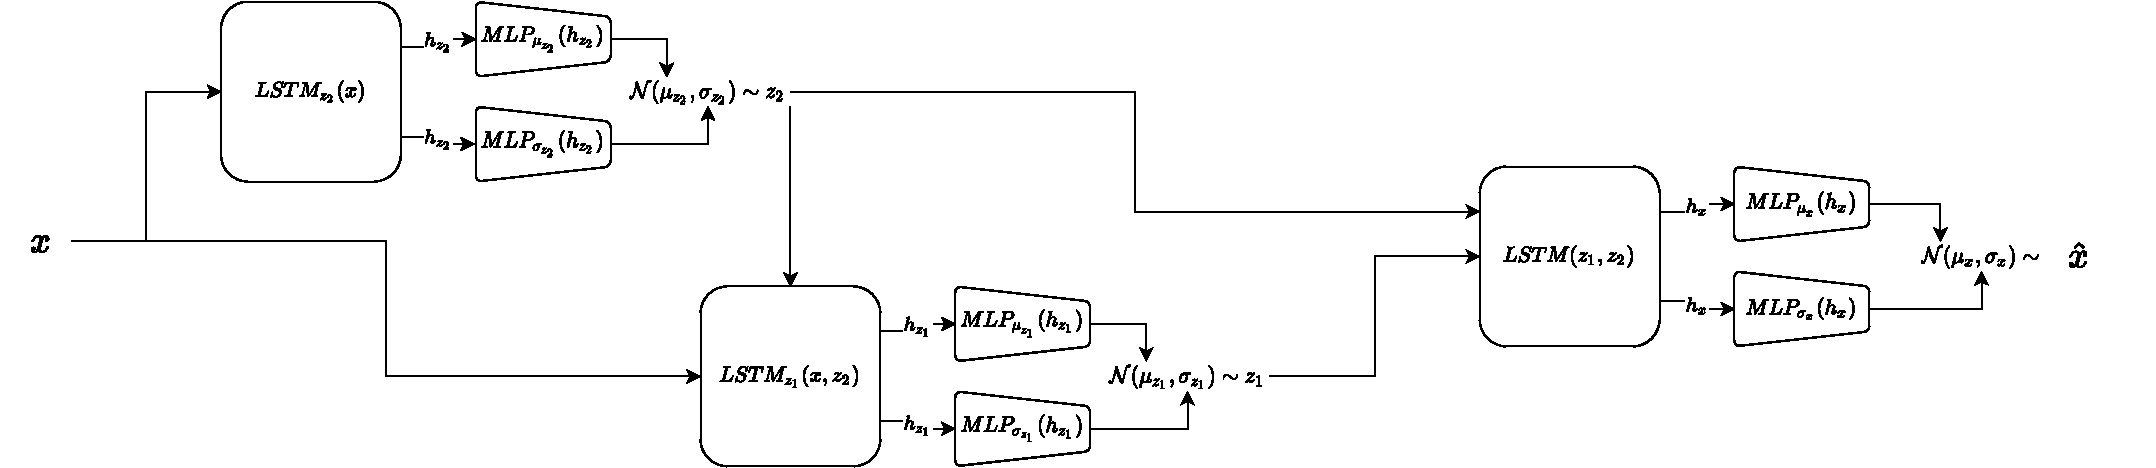
\includegraphics[width=1\linewidth]{../figures/fhvae_complete.pdf}
	\caption{The architecture of the proposed FHVAE. The latent segment variable $z_2$ is conditioned on latent sequence variable $z_1$. Together, they are decoded to parameterize a normal distribution over a reconstructed input $\hat{x}$.}
	\label{fig:fhave}
\end{figure} 
To find an equivariant map for the sequential data setting, \citet{hsu2017unsupervised} propose the FHVAE (see Figure~\ref{fig:fhave}). Its encoder maps to a latent subspace factorized into a latent sequence variable $z_1$ and a latent segment variable $z_2$. To form Gaussian distributions over these latent variable, \citet{hsu2017unsupervised} pass an input sequence $x$ to two distinct Long short-term Memory (LSTM) \cite{hochreiter1997long} cells $LSTM_{z_1}$ and $LSTM_{z_2}$. The hidden states of those cells are decoded by Multi-layer Perceptrons (MLP) to give the mean and standard deviation for each latent variable. To decode the latent space, a sample is drawn and passed to another LSTM. This LSTMs hidden state is decoded to form a normal distribution over a reconstructed input $\hat{x}$.\\
To train the FHVAE, \citet{hsu2017unsupervised} propose a segment variational lower bound, based on \citet{kingma2013auto} and add a discriminative objective. This segment variational lower bound can be written as
\begin{align*}
\mathcal{L}(\theta, \phi, X)& = %\sum_{n=1}^N \mathcal{L}(\theta, \phi;x^{(n)}|\tilde{\mu_2}) + log\;p_{\theta} + const.\\
%\mathcal{L}(\theta, \phi;x^{(n)}|\tilde{\mu_2}) &= 
\underbrace{log\;p(x|z_1, z_2)}_{\text{reconstruction}}\\%prob. of obs. data under learned posterior\\
-&\underbrace{D_{KL}(\mathcal{N}(\mu_{z_1}, \sigma_{z_1})||\mathcal{N}(0,1))}_{\text{regularize $z_1$ with global prior}}\\
-&\underbrace{D_{KL}(\mathcal{N}(\mu_{z_2}, \sigma_{z_2})||\mathcal{N}(\mu_2,0.5))}_{\text{regularize $z_2$ with seq. dep. prior $\mu_2$}}\\
+&\underbrace{log\;p(\mu_2) \cdot \frac{1}{seq.\;length}}_{\text{scaled prob. of $\mu_2$ under standard Gaussian prior}}, 
\end{align*}
where $\theta$ is the set of decoder parameters, $\phi$ are encoder parameters, and $X$ are training samples. Note that while $z_1$ gets regularized through a standard Gaussian prior, $z_2$ is discouraged to deviate from a Gaussian distribution centered ad $\mu_2$. \citet{hsu2017unsupervised} introduce $\mu_{2}^{(i)}$ as sequence $(i)$-dependent prior to encourage factorization. This sequence-dependent prior can be retrieved through a differentiable lookup table. The discriminative objective 
\begin{align*}
log\;p(sequence\;id^{(i)} | z_2^{(i,n)})& = log\;\frac{p(\mu_{z_2}^{(i,n)}|\mu_2^{(i)})}{\sum^{n}_{j=1}	p(\mu_{z_2}^{(i,n)}|\mu_2^{(j)})}
\end{align*}
is used to build an expressive lookup table, where similarity of sequences is reflected by $\mu_{2}^{(i)}$ close in Euclidean space.\\
\citet{hsu2017unsupervised} refer to the resulting objective
\begin{align*}
\mathcal{L}^{dis}(\theta, \phi;x)& = \mathcal{L}(\theta, \phi, X) + \alpha \cdot log\;p(sequence\;id | z_2)
\end{align*}
as discriminative segment variational lower bound, where hyperparameter $\alpha$ determines the weight of the discriminative objective.



\begin{figure}[t]\scriptsize
	% This file was created by tikzplotlib v0.9.8.
\begin{tikzpicture}

\definecolor{color0}{rgb}{0.161,0.2,0.361}
\definecolor{color1}{rgb}{0.937,0.463,0.478}
\definecolor{color2}{rgb}{0.953,0.655,0.0706}

\begin{groupplot}[group style={group size=2 by 2}]
\nextgroupplot[
height=\figheight,
legend cell align={left},
legend style={
  fill opacity=0.8,
  draw opacity=1,
  text opacity=1,
  at={(0.03,0.97)},
  anchor=north west,
  draw=white!80!black
},
tick align=outside,
tick pos=both,
width=\figwidth,
x grid style={white!69!black},
xmin=-0.238, xmax=4.99,
xtick style={color=black},
y grid style={white!69!black},
ymin=-2, ymax=5,
ytick style={color=black}
]
\addplot [semithick, color0, dash pattern=on 1pt off 1pt]
table {%
0 0.6
0.25 0.353
0.5 0.121
0.75 -0.0816
1 -0.241
1.25 -0.349
1.5 -0.397
1.75 -0.384
2 -0.309
2.25 -0.178
2.5 0.00153
2.75 0.218
3 0.459
3.25 0.708
3.5 0.951
3.75 1.17
4 1.36
4.25 1.49
4.5 1.58
4.75 1.6
};
\addlegendentry{Signal}
\addplot [semithick, color1, dash pattern=on 1pt off 1pt]
table {%
0 0.748
0.25 0.282
0.5 0.11
0.75 -0.00702
1 -0.221
1.25 -0.309
1.5 -0.42
1.75 -0.274
2 -0.3
2.25 -0.115
2.5 0.009
2.75 0.244
3 0.375
3.25 0.699
3.5 0.704
3.75 1.16
4 0.797
4.25 1.04
4.5 1.46
4.75 1.49
};
\addlegendentry{Decoder reconstruction}
\addplot [semithick, color2, dash pattern=on 1pt off 1pt]
table {%
0 -3.64
0.25 -3.43
0.5 -3.24
0.75 -3.07
1 -2.94
1.25 -2.85
1.5 -2.8
1.75 -2.82
2 -2.88
2.25 -2.99
2.5 -3.14
2.75 -3.32
3 -3.52
3.25 -3.73
3.5 -3.94
3.75 -4.12
4 -4.28
4.25 -4.39
4.5 -4.46
4.75 -4.48
};
\addlegendentry{$z_1 \cdot sin(x) + z_2$}

\nextgroupplot[
height=\figheight,
tick align=outside,
tick pos=both,
width=\figwidth,
x grid style={white!69!black},
xmin=-0.238, xmax=4.99,
xtick style={color=black},
y grid style={white!69!black},
ymin=-2, ymax=5,
ytick style={color=black}
]
\addplot [semithick, color0, dash pattern=on 1pt off 1pt]
table {%
0 0.6
0.25 0.847
0.5 1.08
0.75 1.28
1 1.44
1.25 1.55
1.5 1.6
1.75 1.58
2 1.51
2.25 1.38
2.5 1.2
2.75 0.982
3 0.741
3.25 0.492
3.5 0.249
3.75 0.0284
4 -0.157
4.25 -0.295
4.5 -0.378
4.75 -0.399
};
\addplot [semithick, color1, dash pattern=on 1pt off 1pt]
table {%
0 0.806
0.25 1.15
0.5 1.01
0.75 1.41
1 1.42
1.25 1.48
1.5 1.46
1.75 1.51
2 1.46
2.25 1.28
2.5 1.18
2.75 1.05
3 1
3.25 0.696
3.5 0.527
3.75 -0.424
4 0.927
4.25 1.39
4.5 1.52
4.75 1.74
};
\addplot [semithick, color2, dash pattern=on 1pt off 1pt]
table {%
0 3.61
0.25 3.84
0.5 4.06
0.75 4.24
1 4.39
1.25 4.49
1.5 4.54
1.75 4.52
2 4.45
2.25 4.33
2.5 4.17
2.75 3.97
3 3.74
3.25 3.51
3.5 3.29
3.75 3.08
4 2.91
4.25 2.78
4.5 2.71
4.75 2.69
};

\nextgroupplot[
height=\figheight,
tick align=outside,
tick pos=both,
width=\figwidth,
x grid style={white!69!black},
xmin=-0.238, xmax=4.99,
xtick style={color=black},
y grid style={white!69!black},
ymin=-2, ymax=5,
ytick style={color=black}
]
\addplot [semithick, color0, dash pattern=on 1pt off 1pt]
table {%
0 0.6
0.25 0.847
0.5 1.08
0.75 1.28
1 1.44
1.25 1.55
1.5 1.6
1.75 1.58
2 1.51
2.25 1.38
2.5 1.2
2.75 0.982
3 0.741
3.25 0.492
3.5 0.249
3.75 0.0284
4 -0.157
4.25 -0.295
4.5 -0.378
4.75 -0.399
};
\addplot [semithick, color1, dash pattern=on 1pt off 1pt]
table {%
0 0.128
0.25 1.01
0.5 0.848
0.75 1.26
1 1.34
1.25 1.44
1.5 1.51
1.75 1.46
2 1.27
2.25 1.29
2.5 1.2
2.75 1.09
3 0.533
3.25 0.632
3.5 0.184
3.75 -0.356
4 0.617
4.25 0.364
4.5 -0.806
4.75 1.4
};
\addplot [semithick, color2, dash pattern=on 1pt off 1pt]
table {%
0 3.71
0.25 3.72
0.5 3.73
0.75 3.75
1 3.75
1.25 3.76
1.5 3.76
1.75 3.76
2 3.76
2.25 3.75
2.5 3.74
2.75 3.73
3 3.71
3.25 3.7
3.5 3.69
3.75 3.67
4 3.66
4.25 3.66
4.5 3.65
4.75 3.65
};

\nextgroupplot[
height=\figheight,
tick align=outside,
tick pos=both,
width=\figwidth,
x grid style={white!69!black},
xmin=-0.238, xmax=4.99,
xtick style={color=black},
y grid style={white!69!black},
ymin=-2, ymax=5,
ytick style={color=black}
]
\addplot [semithick, color0, dash pattern=on 1pt off 1pt]
table {%
0 1.2
0.25 1.2
0.5 1.2
0.75 1.2
1 1.2
1.25 1.2
1.5 1.2
1.75 1.2
2 1.2
2.25 1.2
2.5 1.2
2.75 1.2
3 1.2
3.25 1.2
3.5 1.2
3.75 1.2
4 1.2
4.25 1.2
4.5 1.2
4.75 1.2
};
\addplot [semithick, color1, dash pattern=on 1pt off 1pt]
table {%
0 0.994
0.25 1.34
0.5 0.843
0.75 1.12
1 1.26
1.25 1.1
1.5 1.17
1.75 1.41
2 1.3
2.25 1.05
2.5 1.23
2.75 1.12
3 0.245
3.25 0.529
3.5 0.216
3.75 0.569
4 -0.36
4.25 -0.0586
4.5 -1.44
4.75 1.62
};
\addplot [semithick, color2, dash pattern=on 1pt off 1pt]
table {%
0 2.52
0.25 2.35
0.5 2.19
0.75 2.05
1 1.94
1.25 1.86
1.5 1.83
1.75 1.84
2 1.89
2.25 1.98
2.5 2.11
2.75 2.25
3 2.42
3.25 2.59
3.5 2.76
3.75 2.91
4 3.04
4.25 3.14
4.5 3.19
4.75 3.21
};
\end{groupplot}

\end{tikzpicture}
%
	\centering
	\caption{Sample signals reconstructed with the FHVAE. Blue lines are generated using the latent variables $z_1$ and $z_2$ with the known generative process used to create the training data. For these samples, the latent variables do not correspond to the actual generative factors values.}
	\label{fig:samples}
\end{figure}



\section*{Discussion and Future Work}
\citet{hsu2017unsupervised} evaluate the FHVAE on different tasks. They propose an unsupervised speaker verification task to measure performance, and to some extent, quantitatively assess the grade of disentanglement. They outperform an i-vector baseline \footnote{According to \citet{hsu2017unsupervised}, i-vector is used in state-of-the-art speaker verification approaches. It is a low dimensional subspace of a Gaussian mixture universal background model which ideally only contains speaker information.}. To identify speakers, they use $\mu_2$ which ideally should only encapsulate speaker-dependent attributes. As a sanity check, they further introduce a segment vector $\mu_1$. This variable is based on $z_1$ and should thus ideally only contain information independent of the speaker. The results are displayed Table~\ref{tab:eer}.
\begin{table}[t]
	\caption{Comparison of speaker verification equal error rate (EER) on the TIMIT test set.}
	\centering
	\begin{tabular}{llll}
		\toprule
		Method 				& Dimension 	& $\alpha$ 		& EER  				 \\
		\midrule\midrule
		\multirow{1}{*}{i-vector}
		& 100   & -     & 9.52\%    \\
		\midrule
		\multirow{1}{*}{$\bm{\mu}_2$}  	& 32			& $10^1$	& \textbf{2.38\%}  	 	\\
		\midrule
		\multirow{1}{*}{$\bm{\mu}_1$}
	& 32			& $10^1$		& 22.47\%   	\\
		\bottomrule
	\end{tabular}
	\label{tab:eer}
\end{table}
While using $\mu_2$ results in the lowest EER, they still achieve below random-baseline EER using $\mu_1$, indicating leakage of sequence-level information into $z_1$. This observation reveals a larger problem. While \citet{hsu2017unsupervised} provide visual and audio qualitative examples to demonstrate the grade of disentanglement, they fail in providing sufficient quantitative evidence. Moreover, their work lacks a formal description and justification of the proposed factorization.\\
%TODO elaborate on toy example 
To further investigate the level of disentanglement, we evaluate the FHVAE on a toy dataset with a known generative process. While achieving good reconstruction of signals, the latent variables are not reflective of the generative factors. Sample results are shown in Figure~\ref{fig:samples}.\\
To improve disentanglement, we propose to further exploit the used data by introducing a cross-reconstruction loss \cite{schonfeld2019generalized}. Additionally, we hypothesize that using a hierarchical activation function, as proposed by \citet{shen2018ordered} could further encourage a clean factorization.




\section*{Conclusion}
\citet{hsu2017unsupervised} propose an architecture suited to approximate an equivariant map with respect to a sequence-segment decomposition. They exploit the hierarchical nature of certain sequential data to form an inductive bias towards factorization of different temporal scales. We hypothesize that the notion of a sequence-dependent prior could be transferred to other settings. While achieving good performance on considered benchmark tasks, their work lacks quantitative evidence of achieved disentanglement.
We advocate for the need for more foundational, formal work on disentanglement. We hypothesize that this would allow to fairly discuss, evaluate and compare methods. Otherwise, this emerging field might get ahead of itself, proposing elaborate architectures without sufficient formal frameworks, metrics, and baseline methods. 



\newpage
\bibliographystyle{unsrtnat}
\bibliography{refs}

\end{document}
